\section{Opaque Funds} \label{sec:endogenous}
This section introduces the fund opacity, $\omega_{s}>0$, and demonstrates that belief-driven mltiple equilibria show up regarding the trading strategy of the fund. We discuss economic implications drawn from the equilibrium analyses in Subsection \ref{ss:implications}.

%===========================================
\subsection{Delegation under Fund Opacity}\label{subsec:opaquedelegate}
Assuming that $\omega_{s}>0$, the analysis of an opaque fund largely follows the benchmark case in Section \ref{sec:Model}. In particular, investors' optimization and the structure of the resulting fund flow are identical to those in (\ref{eq:symmetricm}) and (\ref{eq:M}) in the benchmark model. However, due to the noisy revelation of the fund information, investors' conditional expectation about the fund return must be modified as follows:

\begin{lemma}\label{lem:reputation}
	Upon observing the fund information, $x+e$, investors' updated expected trading profit is given by
	\begin{equation}
         \mathrm{E}\left[\pi|x+e\right] = (1-\lambda \beta)\beta\left(\hat{s}^2 + \hat{\omega}_{s}\right),
     \end{equation}
     where the posterior expectation of the (signed) realized skill is
     \begin{equation}
         \hat{s} = \mathrm{E}[s|x+e] = \xi(x+e),
     \end{equation}
     with 
	 \begin{equation}
		\xi = \frac{\beta\omega_{s}}{\beta^2 \omega_{s}+\omega_{e}},\label{eq:xi}
	 \end{equation}
	 and the posterior of the skill variance is
     \begin{equation}
         \hat{\omega}_{s} = \mathrm{Var}[s|x+e] = \frac{\omega_{s}\omega_{e}}{\beta^2 \omega_{s} + \omega_{e}}.
     \end{equation}
 \end{lemma}
 Investors update their belief about the realized skill using $x+e$, where $\xi$ measures how much they rely on the fund information provided by the manager. Holding $\beta$ constant, $\xi$ is large when investors' prior is unreliable ($\omega_{s}$ is large) and the fund information is transparent ($\omega_{e}$ is small). In what follows, the updated expectation about the manager's realized skill, $\hat{s}$, is referred to as the \textit{reputation}.  

 \subsection{Manager's Optimization} \label{ss:optimization_opaque}
Following the same procedures as the transparent benchmark, the manager's optimization problem in (\ref{eq:managerproblem_transparent}) is re-written as follows:
\begin{equation}
	\max_{x}\ sx - \lambda x^2 + \theta(1-\lambda\beta)\beta \left[\xi^2(x^2 + \omega_{e}) + \hat{\omega}_{s}\right].\label{eq:managerproblem opaque}
\end{equation}
As in the baseline model, the first two terms of equation (\ref{eq:managerproblem opaque}) represent the trader's expected trading profit. The third term corresponds to her profits from the fund flow, $M$, which also increases with $|x|$ because she can potentially inflate her reputation $|\hat{s}|$ by placing a large order (either buy or sell).

The unique solution to \eqref{eq:managerproblem opaque} (given $\beta$) is
\begin{equation}
x=F(\beta)s,\label{x}
\end{equation}
where
\begin{equation}
F(\beta)\equiv\frac{1}{2\left(\lambda-\theta(1-\lambda\beta)\beta\xi^{2}\right)}.\label{F}
\end{equation}
$F(\cdot)$ is a nonlinear in $\beta$ because $\lambda$ and $\xi$ are functions of $\beta$. 

%===========================================
\subsection{Equilibrium under Opacity} \label{ss:equilibrium}
The manager optimally chooses \eqref{x} given that the market maker and investors believe that she follows strategy \eqref{x_conj}. In equilibrium, their beliefs must be correct, that is, \eqref{x_conj} and \eqref{x} must be consistent with each other, requiring the following condition:
\begin{equation}
\beta=F(\beta).\label{fixed_point}
\end{equation}
That is, the equilibrium levels of $\beta$ are determined at the fixed points of $F(\cdot)$. Having identified $\beta$, the equilibrium levels of $x$, $p$, and $m$ are determined by equations \eqref{x_conj}, \eqref{eq:p} and \eqref{eq:symmetricm}, respectively. In what follows, we first illustrate the determination of equilibrium $\beta$ through a numerical example, followed by an analytical proposition that formally establishes the equilibria.


\begin{figure}
\centering
\subfigure[Small $\theta$ ($\theta=0.2$) $\Rightarrow$ unique low-$\beta$ equilibrium.]{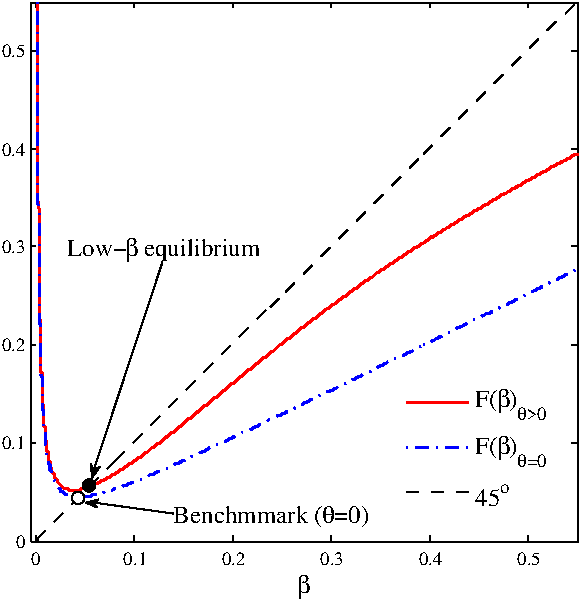
\includegraphics[width=67mm]{./Figures/fig_exogenous_low.pdf}
\label{low}}\quad
\subfigure [Large $\theta$ ($\theta=0.55$) $\Rightarrow$ unique high-$\beta$ equilibrium.]{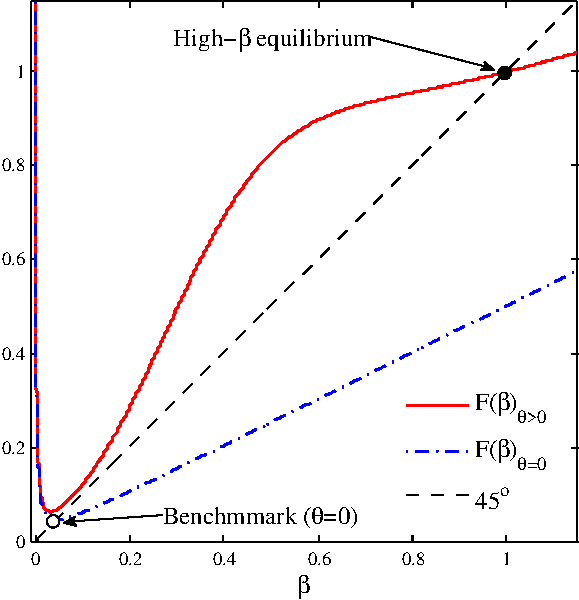
\includegraphics[width=67mm]{./Figures/fig_exogenous_high.pdf}\label{high}}\\[15pt]
\subfigure[Intermediate $\theta$ ($\theta=0.33$) $\Rightarrow$ multiple high-$\beta$ \& low-$\beta$ equilibria.]{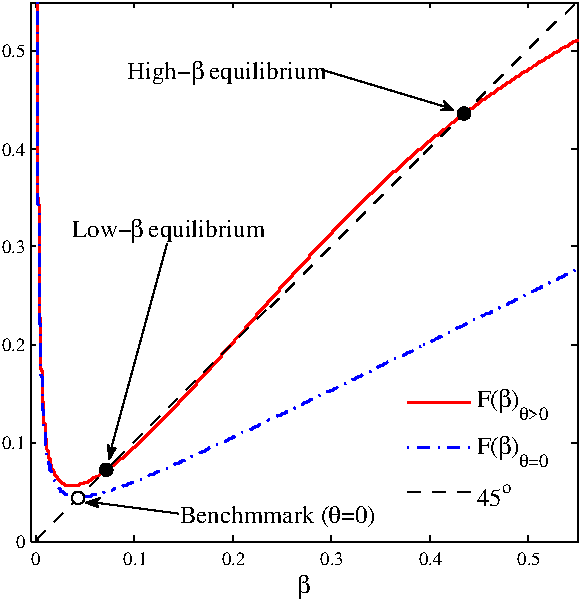
\includegraphics[width=67mm]{./Figures/fig_exogenous_multiple.pdf}\label{multi}}\\[10pt]
\caption{Determination of $\beta$}
\caption*{\footnotesize{Note: The figure plots $F(\beta)$ for different values of $\theta$. The equilibrium values of $\beta$ are determined at the fixed points of $F(\cdot)$.  The parameter values used in the figures are $\omega_{s}=50$, $\omega_{\delta}=1$, and $\omega_{u}=0.1$.}}
\label{fig:exog}
\end{figure}


Figure \ref{fig:exog} illustrates the determination of $\beta$ for three different levels of fund opacity, $\omega_{e}$.
%\footnote{In Figure \ref{fig:exog}, $\omega_{s}$ is assumed to be relatively large. As Proposition \ref{prop:eqm} below formalizes, if $\omega_{s}$ is sufficiently small we do not obtain multiple equilibria as in panel (c) of Figure \ref{fig:exog}.} 
The intersections of $F(\beta)$ (the solid line) and the 45-degree line yield the equilibrium levels of $\beta$. We also plot $F(\beta)$ with $\theta=0$ (the dash-dotted line) and denote its solution as $\beta_{\theta=0}$ to highlight the original model of \citet{kyle1985continuous} where fund delegation is irrelevant.

Panel (a) of Figure \ref{fig:exog} shows that if $\omega_{e}$ is large, there is a unique ``low-$\beta$ equilibrium'' where $\beta$ is close to $\beta_{\theta=0}$. Panel (b) shows that a large $\omega_{e}$ leads to a unique ``high-$\beta$ equilibrium,'' in which $\beta$ is much larger than $\beta_{\theta=0}$.
%\footnote{Formally, we define an equilibrium to be low-$\beta$ (high-$\beta$) if $\beta<\tilde{\beta}$ ($\beta>\tilde{\beta}$), where $\tilde{\beta}$ is defined as square root of the unique solution to equation (\ref{eq:T}) in Lemma \ref{lem:K(1)K(2)} of Online Appendix \ref{proofendogenous}. In the context of Figure \ref{fig:exog}, a low-$\beta$ equilibrium is given by a fixed point of function $F$ at which $F$ is convex and U-shaped, while a high-$\beta$ equilibrium is given by a fixed point that is larger than the first inflection point of $F$. Using this definition, Kyle’s original equilibrium ($\theta=0$) is classified as a low-$\beta$ equilibrium.\label{fn:highlowbeta_def}}
Panel (c) shows that multiple equilibria arise for an intermediate level of $\omega_{e}$. Specifically, the high-$\beta$ and the low-$\beta$ equilibria are stable, as $F(\beta)$ crosses the 45-degree line from above, whereas the one with an intermediate $\beta$ is unstable, as $F(\beta)$ crosses the line from below.\footnote{We define an equilibrium to be stable (unstable) if the corresponding $\beta$ is a stable (unstable) fixed point of $F(\cdot)$, that is, $|F^{\prime}(\beta)|<1$ $(>1)$. A stable equilibrium is robust to a small perturbation to the agents' belief about $\beta$, meaning that the economy converges back to the original equilibrium through the best-response dynamics of the agents' beliefs.}  In what follows, we focus only on the stable equilibria. 

%Panel (a) of Figure \ref{fig:exog} shows that if the trader's reputation concern is weak (i.e., $\theta$ is small), the reputation-driven equilibrium vanishes and only the one close to the benchmark is supported (panel (b)). If the reputation concern is very strong, the Kyle-like equilibrium vanishes and only the one far from the benchmark holds (panel (c)). Multiple equilibria arise if, and only if, the degree of reputation concerns is intermediate (panel (a)). 

\paragraph{\normalfont{\it{Impact of fund opacity.}}}

To see the intuition behind the different equilibrium patterns presented in Figure \ref{fig:exog}, note that the fund manager faces two conflicting motives when trading. On the one hand, she seeks to avoid trading too aggressively on her private information, as doing so would move the price excessively and reduce her trading profits. As in \citet{kyle1985continuous}, this motive leads the trader to decrease $\beta$. On the other hand, she wishes to trade intensively to signal her high skill to her client investors, aiming to establish a strong reputation and attract a large fund flow. This motive encourages her to increase $\beta$. In summary, she faces a tradeoff between ``hiding'' her skill from the market maker and ``showing it off'' to her clients. The fund opacity, $\omega_{e}$, governs this tradeoff by influencing the sensitivity of the manager's reputation, $\hat{s}$, to her investment behavior, $x$. In particular, Lemma \ref{lem:reputation} demonstrates that the fund flow becomes insensitive to $x$ under opacity, as it becomes difficult for investors to estimate the skill based on the fund information, weakening the showing-off motive.

For a opaque fund with a large $\omega_{e}$ (panel (a)), the hiding motive dominates the showing-off motive, leading to a unique low-$\beta$ equilibrium. In this equilibrium, client investors believe that the manager's trading intensity is relatively low. Knowing this, the manager could inflate her reputation by placing an order larger than what her clients anticipates. However, she would refrain from doing so because it would cause a large price impact, reducing the fund's investment profits. Consequently, the equilibrium $\beta$ is close to $\beta_{\theta=0}$, meaning that it is a ``Kyle-like equilibrium." 

For a transparent fund with a small $\omega_{e}$ (panel (b)), the showing-off motive prevails, resulting in a unique high-$\beta$ equilibrium. In this equilibrium, the manager is willing to move the price substantially, undermining investment profits to appear skilled. Importantly, client investors' learning is not manipulated, as their belief about the manager's trading strategy is correct. Nonetheless, the manager places a large order because doing otherwise would induce her clients to incorrectly estimate that she is less skilled, thereby deteriorating her reputation. She trades aggressively solely to conform to her clients' belief. To emphasize this mechanism, we call this equilibrium the ``reputation-driven equilibrium."

For intermediate levels of $\omega_{e}$ (panel (c)), there is no clear dominance between the two motives, hence both the low-$\beta$ and the high-$\beta$ equilibria are supported under intermediate fund opacity. Each equilibrium is associated with a self-fulfilling belief of the market maker and investors.

The following proposition and Figure {\ref{fig:theta}} summarize the above discussion and provide an analytical characterization of the equilibria.

\begin{figure}[t]
    \centering
    \begin{tikzpicture}[scale=2.0]

    % Axes
    \draw[thick,->] (0,0) -- (5,0) node[below] {$\omega_{s}$};
    \draw[thick,->] (0,0) -- (0,3) node[left] {$\theta$};
    % Fill below theta_L and right of threshold with dots
    \fill[pattern=dots, pattern color = black!25] 
        (0,0) to [out = 55, in = 190, looseness=1.2](4.8,2.8)
        -- (4.8, 0)
        to (0,0)
        -- cycle;
    % Fill by gray
    \fill[gray!20] 
        (0.765,1.) to [out = 25, in = 182, looseness=0.5](4.8,1.4)
        -- (4.8,2.8)
        to [out = 190, in = 49, looseness=1.02] (0.765,1.)
        -- cycle;
    % Curves
    %\draw[thick, blue, domain=0:4.8, samples=300] plot (\x, {0.08*(-(\x)^2 + 12*(\x)}) node[right] {$y = x^{0.3}$};
    \draw[thick] (0,0) to [out = 55, in = 190, looseness=1.2](4.8,2.8);
    \draw[thick] (0.765,1.) to [out = 25, in = 182, looseness=0.5](4.8,1.4);
    
    
    
    

    

        
    % Labels
    \node at (1.0,2.4) {\footnotesize High-$\beta$ equilibrium};
    \node at (3,1.8) {\footnotesize Multiple equilibria};
    \node at (2.9, 0.5) {\footnotesize Low-$\beta$ equilibrium};
    

    % Points at the end of curves
    \node[right] at (4.8,2.8) {$\theta_H$};
    \node[right] at (4.8,1.4) {$\theta_L$};

    % Threshold for multiple eqm
    \draw[thick,dashed] (0.77,1.) -- (0.765,0) node[below] {$\tilde{\omega}_{s}$};

    \end{tikzpicture}
    \caption{Equilibrium Characterization with Exogenous $\theta$}
    \caption*{\footnotesize{Note: This figure illustrates the equilibrium states using the reputation concern, $\theta$, and the skill potential, $\omega_{s}$.}}
    \label{fig:theta}
\end{figure}

\begin{proposition}[Equilibrium characterization]\label{prop:eqm}
There exists a critical value of the fund opacity, $\tilde{\omega}_{e}=8\omega_{u}$, and two thresholds of the flow-performance sensitivity, $\theta_{L}$ and $\theta_{H}$ ($\ge \theta_{L}$), such that,
\begin{enumerate}[label=(\roman*)]
	\item if $\omega_{e}\leq \tilde{\omega}_{e}$, then $\theta_{L}=\theta_{H}=\theta_{0}$, and the low-$\beta$ equilibrium uniquely arises when $\theta<\theta_{0}$, while the high-$\beta$ equilibrium uniquely arises when $\theta>\theta_{0}$; and 
	\item if $\omega_{e}> \tilde{\omega}_{e}$, then $\theta_{H}>\theta_{L}$. $\theta> \theta_{H}$ leads to a unique high-$\beta$ equilibrium, $\theta\leq\theta_{L}$ leads to a unique low-$\beta$ equilibrium, and $\theta\in(\theta_{L},\theta_{H})$ leads to multiple equilibria.
\end{enumerate}
\end{proposition}

%Together with the fund opacity, $\omega_{e}$, the flow-performance sensitivity, $\theta$, also influences the equilibrium characterization, as it determines the importance of the fund inflow and thus the reputation in the manager's utility. Proposition \ref{prop:eqm} demonstrates that combinations of a sufficiently opaque fund ($\omega_{e}>\tilde{\omega}_{e}$) and intermediate values of flow-performance sensitivity ($\theta_{L}<\theta<\theta_{H}$) bring about multiple equilibria. As explained earlier, opacity leads to the manager's conflicting motives to trade intensively. When $\theta$ is intermediate, the fund flow is moderately significant in the manager's utility, thereby eliminating a clear dominant strategy for the manager.
\paragraph{\normalfont{\it{Impact of flow-performance sensitivity.}}}
Proposition \ref{prop:eqm} and Figure \ref{fig:theta} indicate that, for a given fund opacity, $\omega_{e}$, a weak flow-performance sensitivity supports only the low-$\beta$ equilibrium, while increases in $\theta$ can generate the high-$\beta$ equilibrium, potentially leading to multiple equilibria.\footnote{Lemma \ref{lem:theta_s} in Online Appendix \ref{proofendogenous} analytically characterizes the upward-sloping $\theta_{H}$ and $\theta_{L}$ in relation to $\omega_{e}$, as presented in Figure \ref{fig:theta}.} To understand intuition, the tradeoff between hiding and showing-off motives, as explained above, is key. 
%On the one hand, she seeks to avoid trading too aggressively on her private information, as doing so would move the price excessively and reduce her trading profits. On the other hand, she wishes to trade intensively to show off her skill to the recruiter. 
When $\theta$ is small, the fund flow's reaction to changes in the expected investment profit becomes weak. In this case, the manager’s showing-off motive is less important. Consequently, the hiding motive prevails, prompting her to trade less aggressively and leading to the low-$\beta$ equilibrium. Conversely, when $\theta$ is large, the fund flow becomes highly sensitive to the fund information, thereby encouraging the manager to show off her skill by trading intensively. This scenario gives birth to the high-$\beta$ equilibrium.

Overall, the type of equilibrium depends on the combination of $\theta$ and $\omega_{e}$, as illustrated in Figure \ref{fig:theta}. The tradeoff between the hiding and the showing-off motive tends to balance and generates multiple equilibria when the fund is relatively opaque, and the fund flow is moderately sensitive to the expected investment performance. Otherwise, one of the conflicting motives dominates the other either because of a sufficiently transparent fund, encouraging the manager to show off her skill, or the fund flow being very sensitive or insensitive to the expected performance, altering the importance of the fund flow relative to the investment profit in the manager's optimization.

\paragraph{\normalfont{\it{Equilibrium comparison.}}}
Comparing the two stable equilibria, does the manager perform better in one of them? What are the implications for market liquidity, asset prices, and learning about asset-selection skills? 
%The following corollary summarizes the results.
\begin{corollary}[High-$\beta$ vs.\ low-$\beta$ equilibrium]\label{cor:high_vs_low}
In the high-$\beta$ equilibrium, relative to the low-$\beta$ equilibrium,
\begin{enumerate}[label=(\roman*)]
\item \label{item:1} the market liquidity is higher, that is, $\lambda$ is lower;
\item \label{item:2} the manager's expected trading profit given the realized skill, $\mathrm{E}[(\delta-p)x|s]=\frac{\beta\omega_{u}s^{2}}{\beta^{2} \omega_{s}+\omega_{u}}$, is lower;
\item \label{item:3} the price informativeness, $\tau\equiv\frac{1}{\mathrm{Var}[\delta|p]}=\frac{\beta^{2} \omega_{s}+\omega_{u}}{\omega_{\delta}(\beta^{2} \omega_{s}+\omega_{u})+\omega_{u} \omega_{s}}$, is higher;
\item \label{item:4} the price volatility, $\mathrm{Var}[p]=\frac{\beta^{2}\omega_{s}^{2}}{\beta^{2} \omega_{s}+\omega_{u}}$, is higher; and
\item \label{item:5} investors' estimate of $s$ is more precise, that is, the posterior variance of $s$, $\hat{\omega}_{s}=\frac{\omega_{s}\omega_{u}\omega_{\delta}}{\omega_{s}(\beta^{2}\omega_{\delta}+\omega_{u})+\omega_{u}\omega_{\delta}}$, is lower.
\end{enumerate}
\end{corollary}

Statement \ref{item:1} of Corollary \ref{cor:high_vs_low} holds because price impact $\lambda$ is decreasing in $\beta$ in the equilibrium. Since the high-$\beta$ equilibrium emerges only if $\theta$ is relatively large, the statement also implies that a higher flow-performance sensitivity leads to higher market liquidity. The intuition is as follows. Relative to the low-$\beta$ equilibrium, in the high-$\beta$ equilibrium the manager trades more aggressively, and thus the order flow reflects significant information about $s$. To incorporate the appropriate amount of information about $s$ into the price, the market maker seeks to offset the exaggerated information in order flow by lowering $\lambda$.

The intuition for statement \ref{item:2} is closely related to that for statement \ref{item:1}. In the high-$\beta$ equilibrium, the manager earns a lower trading profit due to a smaller informational advantage over the market maker. This result may appear inconsistent with statement \ref{item:1} because, ceteris paribus, a lower price impact is typically associated with a higher trading profit. However, the manager's order size $|x|$ in the high-$\beta$ equilibrium is so large that the {\it overall} price impact (i.e., $\lambda$ multiplied by $|x|$) is larger than that in the low-$\beta$ equilibrium. Consequently, the manager moves the price excessively and earns a lower trading profit in this equilibrium.
%\footnote{Our numerical result, not presented in the paper but available upon request, indicates that the trader's overall expected utility, including the reputation benefit, is also lower in the high-$\beta$ equilibrium.} 
Due to her aggressive trading, more information about $s$---which is informative about $\delta$---is incorporated into the price in the high-$\beta$ equilibrium, supporting statement \ref{item:3}.

Statement \ref{item:4} follows, again, from the manager's aggressive trading in the high-$\beta$ equilibrium. Specifically, she places a large buy (sell) order when $s>0$ ($s<0$), even if $|s|$ is small. This causes a large upward (downward) pressure on $p$, leading to greater price variability. This result aligns with the insight of \citet{guerrieri2012fund} that reputation concerns amplify price volatility, although their mechanism differs from ours.\footnote{\citet{guerrieri2012fund} argue that bond price volatility increases because fund managers demand a premium to offset the risk of reputation damage in the event of default.}

In the high-$\beta$ equilibrium, the manager reveals more information about $s$, thereby improving the precision of investors' estimation (statement \ref{item:5}). This makes the fund flows more responsive to skill, as investors can assess it more accurately.

%{\color{red} [TO ADD, perhaps, what our model would imply about increasing skill ($\sigma_{s}^2$), an increasing industry, and no improvement in aggregate performance.]}

%{\color{red}[TO ADD HERE, MAYBE: Learning in our model is not based on performance as measured by profits. We have many sources of info, price and payoff, return... but it's not return on its own... it's important for the incentive to move the price]}


%%-------------------------------------------
%\subsubsection{No noise trading}
%Our model also yields a result that is intriguing from a somewhat technical point of view: reputation-driven trades occur even if we do not assume noise traders.
%\begin{corollary}[No noise trading]\label{cor:no_noise_trading}
%Even in the absence of noise traders (i.e., $\sigma_{u}=0$), each trader trades in a stable equilibrium if $\theta>0$. She submits $x=2\thetas$ while the price $p=\hat{\delta}+s$ fully reveals her $s$, and her expected trading profit is $\mathrm{E}[\pi|s]=0$.
%\end{corollary}
%This result contrasts with Kyle (1985) and many other finance models in which trades occur only at the expense of noise traders. In these models, a trader would submit $x=0$ and therefore the market would break down if $\sigma_{u}=0$. The absence of noise traders implies that the market maker knows the exact level of $x$, which fully reveals the trader's information. This is the reason $x=0$ would hold if $\sigma_{u}=0$ in Kyle (1985).\footnote{To see why $x=0$ holds, consider what would happen to our equilibrium if $\theta=0$. Suppose that the market maker believes $x=\betas$ for some $\beta>0$. Then, from \eqref{x}, the trader's best response is to choose $x=F(\beta)s=\frac{1}{2\lambda}s=\frac{\beta}{2}s$. That is, she trades less aggressively than the market maker's belief. She does so in an effort to lead the market maker to underestimate $|s|$ so she can exploit the resulting mispricing. But the market maker would rationally anticipate it. So, suppose that the market maker believes  $x=\frac{\beta}{2}s$. Then the trader's best response is to choose $x=\frac{\beta}{4}s$ for the same reason as above. Continuing this way, the only situation supported as an equilibrium is that the trader chooses $x=0$ and the market maker correctly believes it.} But in our model, the trader chooses $x\neq 0$ due to the reputation concern: if, for whatever reason, the recruiter believes that $\beta>0$, the trader needs to conform with it and submit $x\neq 0$, since otherwise the recruiter would believe ex post that $|s|=0$, leading to zero reputation benefit. She does so while knowing that such a trade will make zero expected profit.

%Our numerical exercises suggest that the trader's unconditional expected utility is higher in the low equilibrium. While the expected reputation gain is increasing in $\beta$, the increase is not high enough to make up for the decrease in profits. We obtain similar results conditional on skill, with the exception that for low skill, $|s|$, trading more aggressively lowers both the expected profit and the expected reputation gain. 

%\subsubsection{Comparative statics} \label{sss:compStat}
%%-------------------------------------------------------------------------------------------------------------------
%[\textbf{Two period model $\theta$ depends on $\sigma_{s}$; perhaps redo the comparative statics analysis? A: Nope, not for now; we could just change \sigma_{u,1}.}]

%[Y: Intuition is unclear.]
%In Figure \ref{fig:CSintermVarEta} we show that trading aggressiveness decreases in the informational advantage of the trader, $\sigma_{s}^{2}$. This holds in price impact models in general: when he is more uncertain about his estimate of the asset payoff, the market maker extracts more information from the order flow and the price impact increases; this forces the trader to reduce her trade in order to protect profits. Due to the conflicting incentive to place a larger order to show off skill, the trader's trade in our model is less sensitive to increases in $\sigma_{s}^2$. As a consequence, we observe an increasing gap between our equilibrium $\beta$ and $\beta_{Kyle}$.  As uncertainty about private information increases further, the low-$\beta$ equilibrium emerges, while the high-$\beta$ one continues to exist. Similar to the Kyle equilibrium, the low-$\beta$ one is more sensitive to further changes in $\sigma_{s}^2$.
%\textit{With lower reputation concerns, as measured by $\theta$, the economy seems less fragile, in the sense that the equilibrium is unique. However, looking at the properties of the equilibrium $\beta$ as we vary $\sigma_{s}^2$, we notice that for lower values of payoff/skill uncertainty, trading aggressiveness is less responsive than in Kyle, while the opposite is true for larger values. The former behavior corresponds to the high equilibrium, the latter, to the low equilibrium.}[\textbf{We see this from the increasing and then decreasing gap between $\beta_{Kyle}$ and our $\beta$. Not able to say exactly what's the mechanism behind this, but I'm writing it nevertheless, could be useful later when/if we look at this analysis more carefully.}]

%\bigskip
%\centerline{\bf [Place Figure~\ref{fig:CSintermVarEta} about here]}
%\bigskip

%[Y: Intuition is unclear.]
%In Figure \ref{fig:CSintermVarU} we observe that trading aggressiveness increases with $\omega_{u}$ in the low equilibrium and decreases with $\omega_{u}$ in the high equilibrium. The low equilibrium emerges as noise trading uncertainty increases and it becomes the unique one \textit{relatively fast}. The decreasing gap between $\beta$-low and $\beta_{Kyle}$ shows that our equilibrium is relatively less sensitive to this parameter.  %Relative weight, more noise in the order flow, less weight on it, relative to the payoff. What would happen in a model with only one signal? Contrast the results. Both equilibria exist as the volatility increases further, but for large values uniqueness obtains at the low equilibrium. 

%\bigskip
%\centerline{\bf [Place Figure~\ref{fig:CSintermVarU} about %here]}
%\bigskip

%[Y: This paragraph is potentially interesting. Need to elaborate much more carefully and clearly, probably using a graph with \sigma_{\delta} on the horizontal axis.]
%The residual uncertainty in the asset payoff, $\omega_{\delta}$, only impacts trading aggressiveness in the model with reputation concerns. Figure \ref{fig:CSintermVarEps} shows that as uncertainty increases, so does $\beta$. The result is intuitive, since more noise in the realized payoff makes the market place more weight on the price when updating its beliefs about skill. This in turn increases the trader's incentive to influence beliefs through larger trades. 

%\bigskip
%\centerline{\bf [Place Figure~\ref{fig:CSintermVarEps} about here]}
%\bigskip

%As $\omega_{\delta}$ increases, (1) $\beta$ increases, so profit considerations allow the low equilibrium to continue to exist; (2) the incentives to influence beliefs are so high, that the high equilibrium emerges; we therefore obtain multiple equilibria for `intermediate' values of $\omega_{\delta}$. With further increases the high equilibrium stops satisfying the second order condition and the low equilibrium disappears altogether. With a higher degree of reputation concerns, $\theta$, the high equilibrium survives for larger values of $\omega_{\delta}$.  % more fragility with higher theta? range with multiple equilibria + existence of high eqm 

%===========================================
%[Y: This section looks interesting, but needs much more careful explanations so the first-time readers would understand. Even I don't understand it well.]
%\subsection{Discussion}
%We can interpret increases in the uncertainty about skill $\sigma_{s}^{2}$ as having more skilled traders/traders in the capital markets industry, an inflow of skilled labor in financial services; conversely, an outflow of skilled traders would be associated with a decrease in $\sigma_{s}^{2}$. We would therefore expect to see fragility (multiple equilibria) in markets with more skilled traders (or alternatively, where the informational advantage of the traders is higher). Along the high equilibrium, inflows of skill are good for price informativeness: more information is incorporated into prices relative to the Kyle-equilibrium. % recall high eqm less sensitive, so even though beta decreases with sigma_eta, it does so at a lower pace
%Interestingly, fragility is also likely to occur in markets where there is little uncertainty about noise trading, therefore in markets where there is little uncertainty about fire sales, or large funds rebalancing their portfolios. % low sigmaU for multiple equilibria 
%Similarly, low economic uncertainty or little opacity (as captured by a low $\omega_{\delta}$) is associated with fragility in our model. Along the high equilibrium more residual uncertainty/opacity increases price informativeness. 

%We have established in Section \ref{ss:analysis} that a higher degree of reputation concerns, as captured by the parameter $\theta$, leads to larger trades (corresponding to the high equilibrium). 
%As we show in Section \ref{sec:endogenous}, the degree of reputation concerns $\theta$ depends on both labor market quantities and quantities related to future profit opportunities and independent of the trader's skill. The probability of the trader being hired next period positively impacts $\theta$. Therefore, an increase in this probability, triggered by either an increase in demand or decrease in supply in the labor market, could push the economy to an equilibrium with much more aggressive trading---compare the low-$\beta$ equilibria in panels (a) and (b) of Figure \ref{fig:exog} with the high-$\beta$ equilibrium in panel (c). A similar outcome could be result from greater uncertainty about future liquidity trading or from a shrinking pool of very skilled traders in the future. Both decrease price impact and lead to higher expected future profits and thus a higher expected salary.

% liquidity trading --more uncertainty about fund outflows or fire sales 
% not sure how to interpret a decrease in $\sigma_{s}^{2}$: the component that traders uncover is more likely closer to 0, so skill is more likely zero; could be because public info is of better quality; or the pool of skilled traders is shrinking?